\documentclass[a4paper]{article}

%% Language and font encodings
\usepackage[english]{babel}
\usepackage[utf8x]{inputenc}
\usepackage[T1]{fontenc}
\usepackage{graphicx}
\usepackage{caption}
\usepackage{subcaption}
\usepackage{eurosym}
\usepackage{multirow}
\usepackage{footnote}
\usepackage{listings}
\usepackage{color}
\usepackage{pdfpages}

%% Sets page size and margins
\usepackage[a4paper,top=3cm,bottom=2cm,left=3cm,right=3cm,marginparwidth=1.75cm]{geometry}

%% Useful packages
\usepackage{amsmath}
\usepackage{graphicx}
\usepackage[colorinlistoftodos]{todonotes}
\usepackage[colorlinks=true, allcolors=blue]{hyperref}
\begin{document}

\begin{titlepage}

\newcommand{\HRule}{\rule{\linewidth}{0.5mm}} % Defines a new command for the horizontal lines, change thickness here

\center % Center everything on the page
 
%----------------------------------------------------------------------------------------
%	HEADING SECTIONS
%----------------------------------------------------------------------------------------

\textsc{\LARGE Ecole Polytechnique de Bruxelles}\\[1.5cm] % Name of your university/college
\textsc{\LARGE University of Leeds}\\[1.5cm]
\textsc{\large Johnston Lab Internship}\\[0.5cm] % Minor heading such as course title

%----------------------------------------------------------------------------------------
%	TITLE SECTION
%----------------------------------------------------------------------------------------

\HRule \\[0.4cm]
{ \huge \bfseries Technical description and User guide: Lick-Sensor device for behavioral rodent experiments}\\[0.4cm] % Title of your document
\HRule \\[1.5cm]
 
%----------------------------------------------------------------------------------------
%	AUTHOR SECTION
%----------------------------------------------------------------------------------------

\begin{minipage}{0.4\textwidth}
\begin{flushleft} \large
\emph{Author:}\\
Maxime \textsc{Verstraeten} % Your name
\end{flushleft}
\end{minipage}
~
\begin{minipage}{0.4\textwidth}
\begin{flushright} \large
\emph{Supervisor:} \\
Jamie \textsc{Johnston}\\[0.3cm] % Supervisor's Name
\end{flushright}
\end{minipage}\\[2cm]

% If you don't want a supervisor, uncomment the two lines below and remove the section above
%\Large \emph{Author:}\\
%John \textsc{Smith}\\[3cm] % Your name

%----------------------------------------------------------------------------------------
%	DATE SECTION
%----------------------------------------------------------------------------------------

{\large \today}\\[2cm] % Date, change the \today to a set date if you want to be precise

%----------------------------------------------------------------------------------------

\vfill % Fill the rest of the page with whitespace

\end{titlepage}


\noindent\rule{\textwidth}{1pt}

\tableofcontents

\newpage

\listoffigures

\newpage



\section{Introduction}
This user guide intends to provide the user with the information required to use and understand the lick-sensor device developed at JohnstonLab as well as giving some clues regarding troubleshooting.\\

This device was developed as part of my internship at JohnstonLab (Leeds University, UK) during my master's years as a student engineer from the Université Libre de Bruxelles, Belgium.

This device is part of the rig that allows the lab to perform in-vivo measurements and experiments on mice. This device has been designed to be able to perform behavioral experiments with a reward system in relation to different stimuli such as odors. \\

Note: The workflow, thoughts, issues, ... for this project are discussed in my OneNote.\\

The latest software and documentation updates are available on my Github: \url{https://github.com/maverstr/Lick-Sensor}

\section{Objective}
The lick-sensor device is intended to be use for mice behavioral studies in a kind of reward system with sugared water. The device allows a mouse to lick a needle which shall deliver some water through a valve. The amount delivered can be setup logically with an Arduino code as well as the conditions required for delivery (e.g. the minimum delay between two deliveries, in case of specific odors delivered, ...). 

\section{Hardware}
\subsection{Water Tank}
The water should be stored higher than the delivery as to provide pressure for the water to flow through the valve and as flat as possible to avoid a high change of pressure as the water level drops.
\subsection{Valve}
The chosen valve is a solenoid valve VDW22LA for its size, price and speed of actuation. It is working with 24V DC and as it is a solenoid valve, it will create peak voltage and current when switching it off/on so care must be taken to cope with this issue both on the hardware and software sides.
\subsection{Enclosure}
The device comes with its enclosure which implements a switch for long duration activation of each valve, a push-button each, as well as a BNC input for the olfactometer valve trigger. The valves are connected through 2 XT60 connectors (mounted on the enclosure using a 3D-printed design) and the sensor wires are also connected through their XT60. 3 BNC outputs are available for the licking signal and the 2 valves activation signal.

The box can be seen in CAD in Figures \ref{fig:CAD1} and \ref{fig:CAD2}.

Note: Sensor+ is connected to 9V (hence "+") while Sensor- is connected to ground through a series of resistors. It is NOT a differential signals. Just a denomination for two wires coming onto two different pads on the circuit.

\begin{figure}[h!]
    \centering
    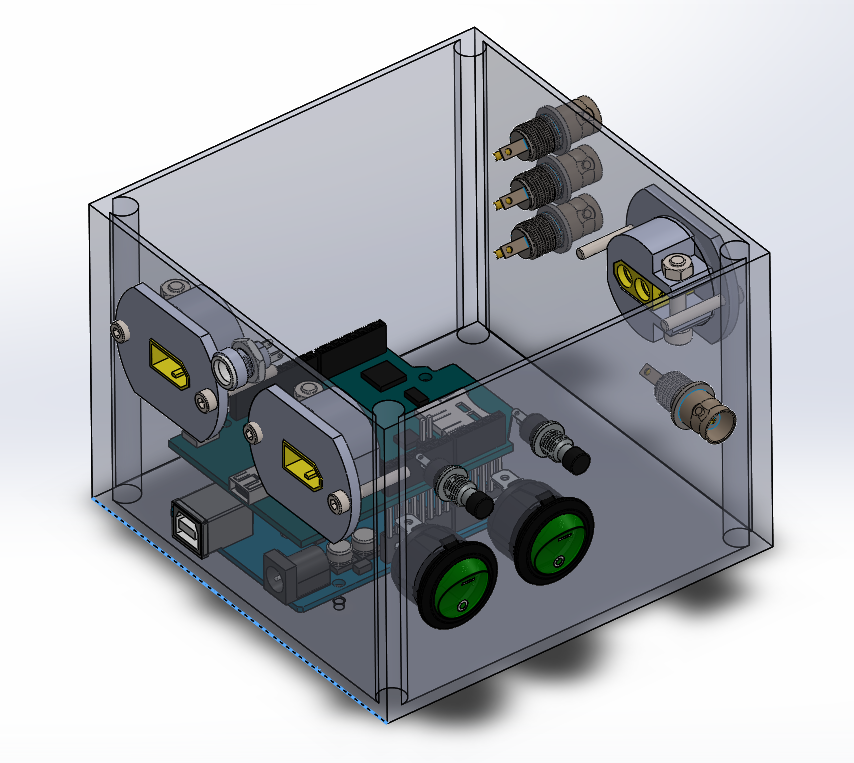
\includegraphics[width = 8cm]{images/CADBox1.png}
    \caption{CAD View: Box design}
    \label{fig:CAD1}
\end{figure}


\begin{figure}[h!]
    \centering
    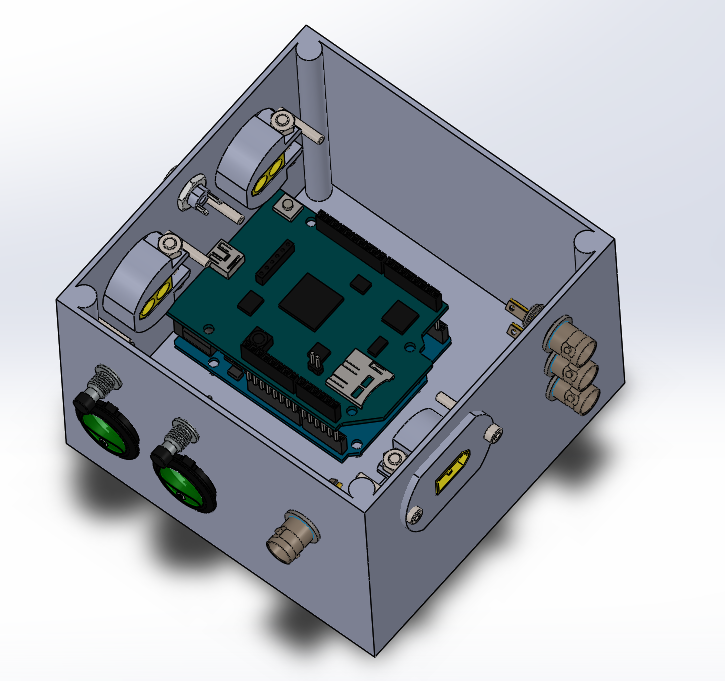
\includegraphics[width = 8cm]{images/CADBox2.png}
    \caption{CAD View: Box design}
    \label{fig:CAD2}
\end{figure}

\begin{figure}[h!]
    \centering
    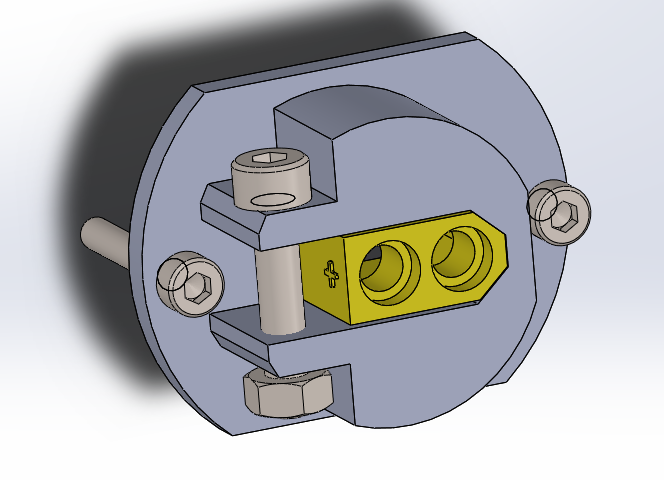
\includegraphics[width = 8cm]{images/xt60Mount.png}
    \caption{CAD View: XT60 panel mount}
    \label{fig:xt60Panel}
\end{figure}

\subsection{Microcontroller}
The µC used is an Arduino Uno. The PCB is designed to be stacked on top of it so that each PCB pin is correctly connected to the Arduino. 

\section{Software}
The Arduino has been programmed using Arduino IDE. 

It works around interrupts setting flags which are being polled every loop of the main loop.
The touch sensor circuit, once powered, provides a 3.3V TLL active low signal connected to pin 2 of the Arduino. Once a falling edge is detected, an interrupt is triggered which sets a flag to True. In the loop, the flag will be reset and, if the conditions are met, an appropriate duration pulse is output to pin 6 and 7 for the valves activation. This 3.3V signal will then be sent to a MOSFET circuit which activates the valve with 24V. This will therefore activate the valve for the specific duration.

It works the same way for the toggle-switches and push-buttons activations (i.e. interrupt, flag, pulse output).

A special mode is available in which the valve is activated trough the touch-sensor only if a reward odor has been sent. The corresponding reward odors pattern must be entered in the code beforehand. 

The drain valve is automatically activated after a set amount of time if a drop is present to suck it back into the pipe.

\section{How to use?}
The device should be powered through the DC socket with a 24V DC supply.
Connect the XT60 connectors to the valves connectors and sensors connectors. The crocodile clamps for the sensors must then be attached on the needle and on the frame connected to the mouse. Obviously, correct polarity must be observed for the valve (Red cable is 24V, black cable is ground for both the wires coming from the PCB and the valve), and it should be trivial with XT60 connectors which are keyed connectors

The valve is activated when both sensors are touched at the same time or when the push-button is pressed or the switch is in up position.

The button can be used to manually set a droplet on the needle, the switch for a long time activation (clearing the water tank, filling the void in the pipes, ...) and the BNC input can be triggered by another script such as a Python script that would randomize odours and associate the odours with a droplet.

To ensure that a single droplet is present on valve activation, you have to calibrate the water flow. This can be done with flow restriction devices clamping the pipes and/or by changing the valve opening duration in the code. The same process must be done for the draining valve to ensure that only the water amount of a droplet is drained.


\section{Electronic Circuits}
\subsection{Sensor circuit}
\subsubsection{Original circuit}
The basic sensor circuit is based of a paper (Slotnick, A simple 2-transistor touch or lick detector circuit, 2009) and allows to send a TTL output (by closing a reed relay) whenever an animal touches two wires at the same time.

\begin{figure}[h!]
    \centering
    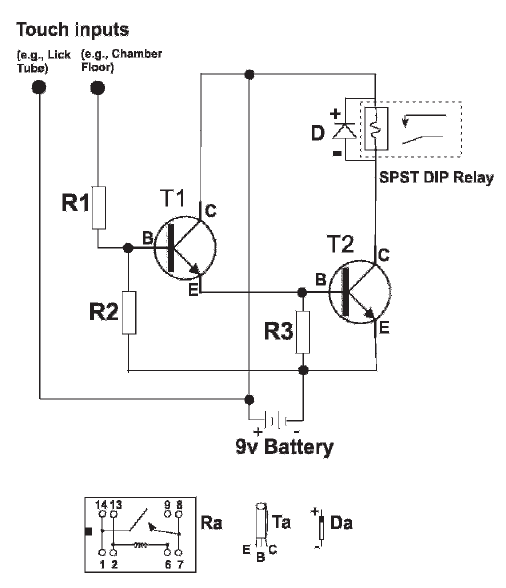
\includegraphics[width = 10cm]{images/sensor.png}
    \caption{Sensor circuit}
    \label{fig:sensor}
\end{figure}

By analysing the paper and the circuit we note that
\begin{itemize}
    \item since the animal subject must survive the experiment and ideally not notice the lick sensor, the current flowing through the rodent should be minimal..
    \item A battery-operated circuit makes it independent from a DC power supply and an AC line and thus does not require isolation transformer (or optocoupler, ...) to protect the rodent.
    \item The circuit proposed here above is using a 9V battery, the current flowing is less than 1µA (according to the paper) and the output operates a relay that can then act as a switch to operate any microcontroller, whatever the voltage required for the logic inputs and therefore not requires level shifting (directly outputs TTL-compatible pulses)
    \item According to the paper, a 9V alkaline battery is sufficient for a couple of months of experiment. 5.5V is the minimum battery voltage for reliable operation. A 9V lithium battery could have an extended lifetime.
    \item The battery could also be replaced by a Zener in 6.3V from a 12 or 24V DC power supply which allows unlimited lifetime and controlled voltage or from a voltage regulator or 9V DC supply.
\end{itemize}

\subsubsection{Actual implementation: First design}
The sensor circuit is only a small part of the whole circuit shown below. Moreover, I decided to add a pull-down at the output of the TTL relay and add some decoupling capacitors on the circuit.
The BJTs used are PN2222A and the relays are COTO 9007-05-01 SPST.

\subsubsection{Actual implementation: Second design}
After testing, It was decided that the relay wasn't reliable enough and expensive.
I designed a new circuit that can switch faster, is cheaper and more reliable.

\begin{figure}[h!]
    \centering
    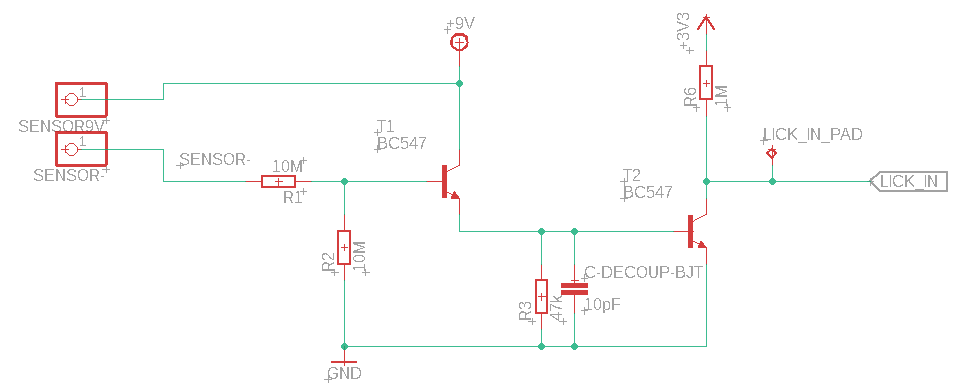
\includegraphics[width = 10 cm]{images/sensorv3.png}
    \caption{Improved sensor circuit}
    \label{fig:sensorv3}
\end{figure}

It has been implemented in the V3 and the circuit can be seen on Figure \ref{fig:sensorv3}.

\subsection{DC/DC Converter}
The valves require 24V DC and the Arduino is powered by 9V on Vin pin. It is then possible to get 5V and 3.3V using the voltage regulators of the Arduino.

To avoid getting a supply for 24V and 9V, a single DC Supply 24V is used and a TSR 1-2490 DC/DC switching regulator is used to provide 9V.
Circuit is shown on Figure \ref{fig:dcdc}.

\begin{figure}[h!]
    \centering
        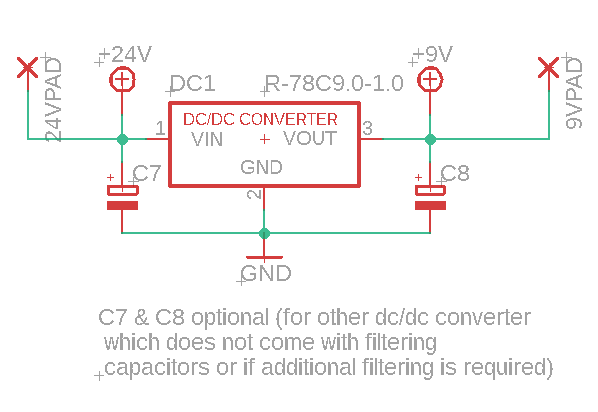
\includegraphics[width = 8cm]{images/dcdcconverter.PNG}
    \caption{DC/DC Converter circuit}
    \label{fig:dcdc}
\end{figure}

Early design implemented linear voltage regulators but they tended to overheat and required the use of a fan.


\subsection{Logical part, µC}
The logical part is handled by an Arduino Uno.

The pinout is shown in Figure \ref{fig:logical}.

\begin{figure}[h!]
    \centering
    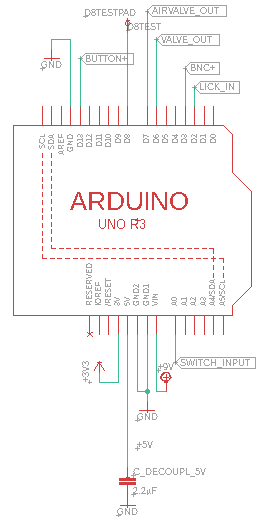
\includegraphics[width = 6cm]{images/logical.PNG}
    \caption{Arduino pinout}
    \label{fig:logical}
\end{figure}

\subsection{Valve Actuator circuit}
\label{actuator}
The valve actuator circuit is composed of a digital input (3.3V, coming from the Arduino digital output pin) which is the Arduino command for opening the valve. R5 and R4 protect the FET gate and provide a way for the gate capacitance to discharge rapidly.

\begin{figure}[h!]
    \centering
    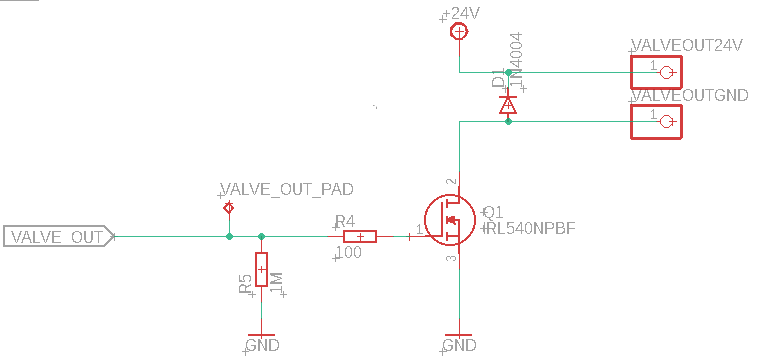
\includegraphics[width = 10cm]{images/actuator.PNG}
    \caption{Valve actuator circuit}
    \label{fig:actuator}
\end{figure}

This part is shown on Figure \ref{fig:actuator}.

When 3.3V signal is given, the FET opens and connects the solenoid valve ground pin to actual ground. Current can then flow through the solenoid and activate the valve. This is basically sinking-current activation.

A fly-back diode is extremely important to protect the circuit against peak voltage when switching the valve off.

An additional Zener diode could be added to the MOSFET gate to protect it against ESD but once in place on the Arduino, the Arduino ESD protection do the trick and there is no risk for normal operation overvoltage as the pin are only capable of outputting 3.3V.


\subsection{Adding a second valve for droplet removal}
It has been discussed later that to be more flexible in behavioral experiments, it would be interesting to add a new valve to drain the droplet that may stay on the needle if the mouse doesn't lick it before a certain time.
Indeed, if the droplet is triggered by an odor and we want to train the mouse to associate this odor with food (or reward, i.e. sugary water) the droplet can't stay (if it isn't licked) and another odor is sent or the mouse will not correctly associate the odors with the correct reward.

To drain the droplet, we must simply open the circuit to air to stop the capillarity effect. The water pipe is therefore connected to a second pipe with the other valve.
This valve is the same as the first one (VDW22LA) as water will flow through to be drained and it reduces the number of different components (Plumbing drawing can be seen on Figure \ref{fig:plumbing}).

\begin{figure}[h!]
    \centering
    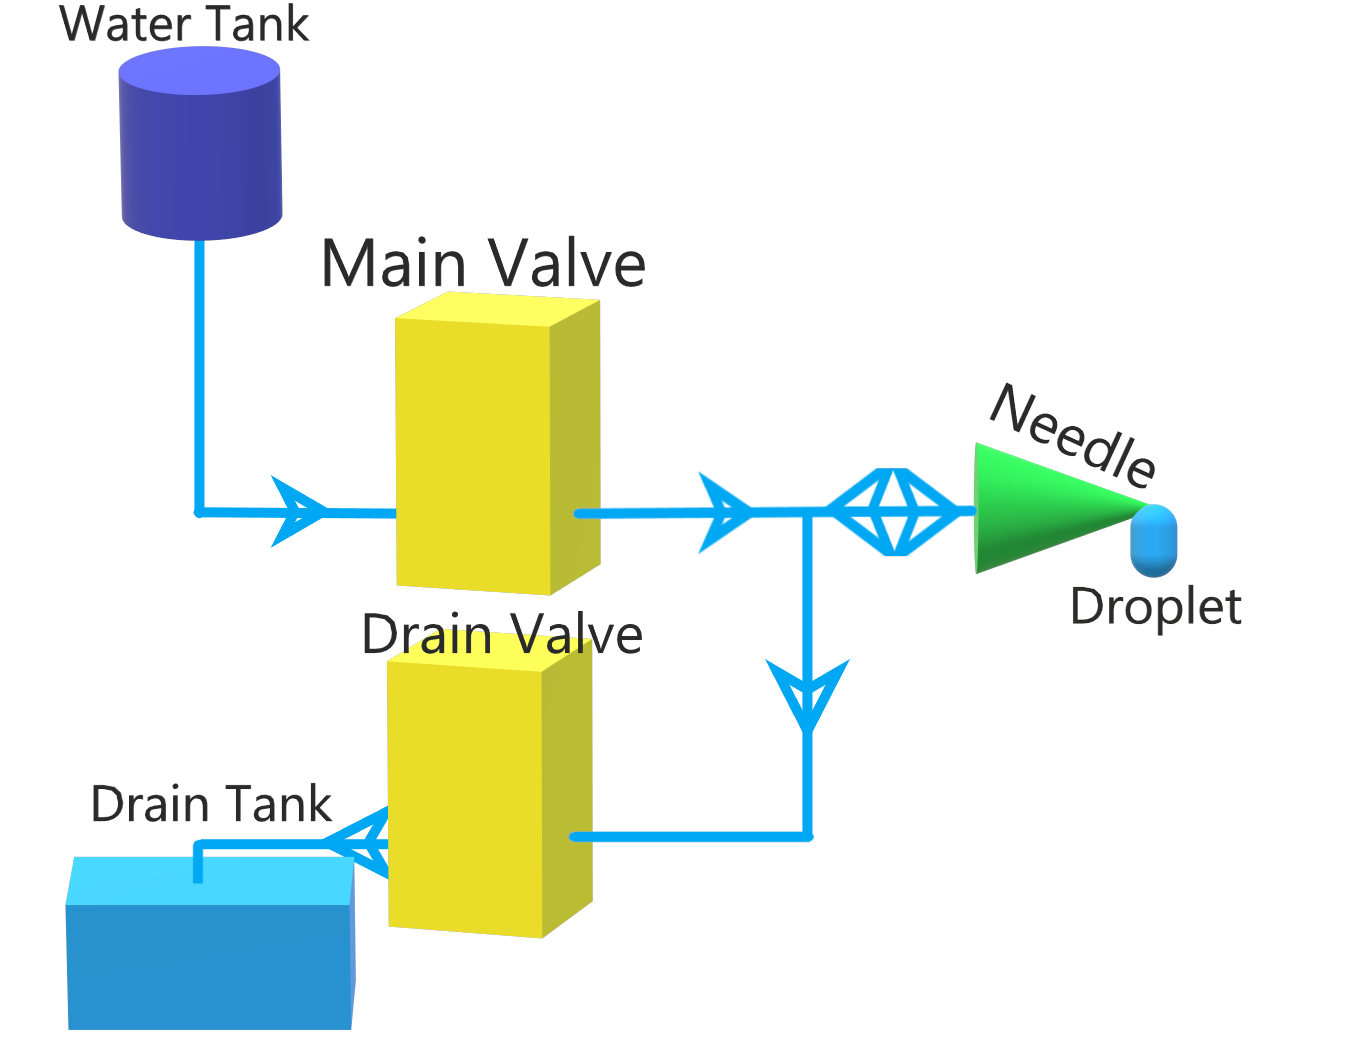
\includegraphics[width =10cm]{images/ValveMap.png}
    \caption{Plumbing Map}
    \label{fig:plumbing}
\end{figure}


This requires to design a second valve circuit actuator. (the same as shown in section \ref{actuator}.
It was the opportunity to implement some of the improvements discussed.

This new design is shown in section \ref{designV3} and the effect is show on video: \url{https://youtu.be/NlbA2PdCB6I}
\newpage
\subsection{Full design V1}
The full circuit has shown some good results but the relays (especially the one driving the valve) is not reliable enough and needs to be replaced every thousand actuations. 
Moreover, this V1 design used linear voltage regulators which tended to overheat.
This design also didn't implemented a direct way to avoid peak voltage on the load. (a snubber RC circuit has been added later on when testing the PCB).

\begin{figure}[h!b!t!]
    \centering
    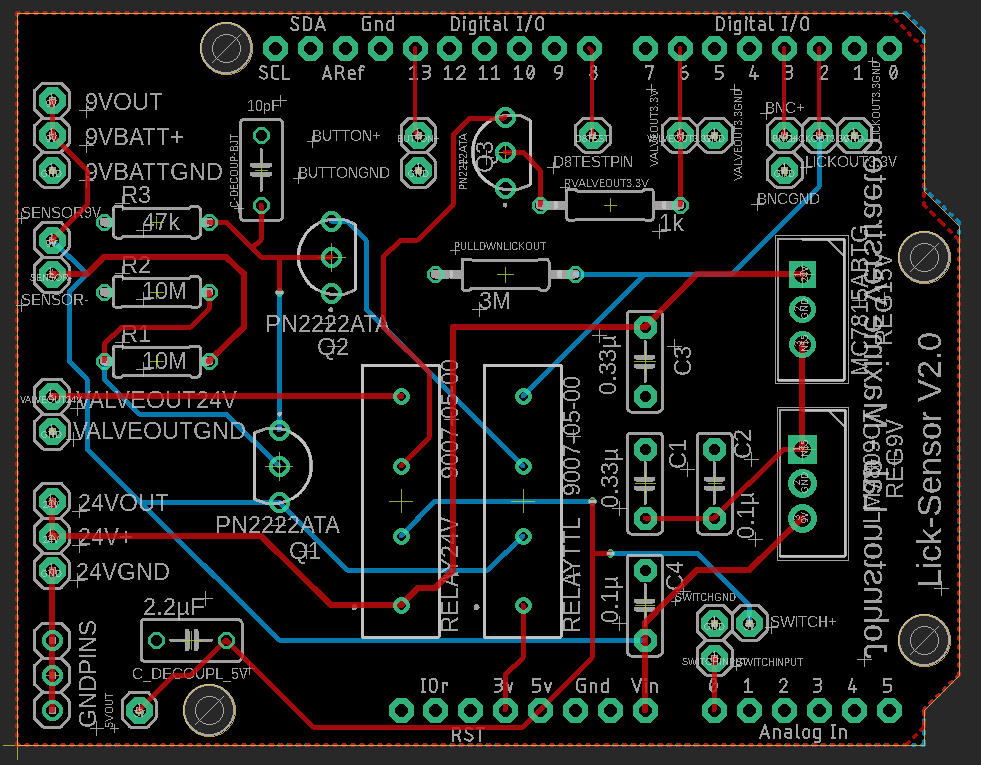
\includegraphics[width = 10cm]{images/schematic.PNG}
    \caption{Design V1: PCB View}
    \label{fig:schematic}
\end{figure}

\begin{figure}[h!b!t!]
    \centering
    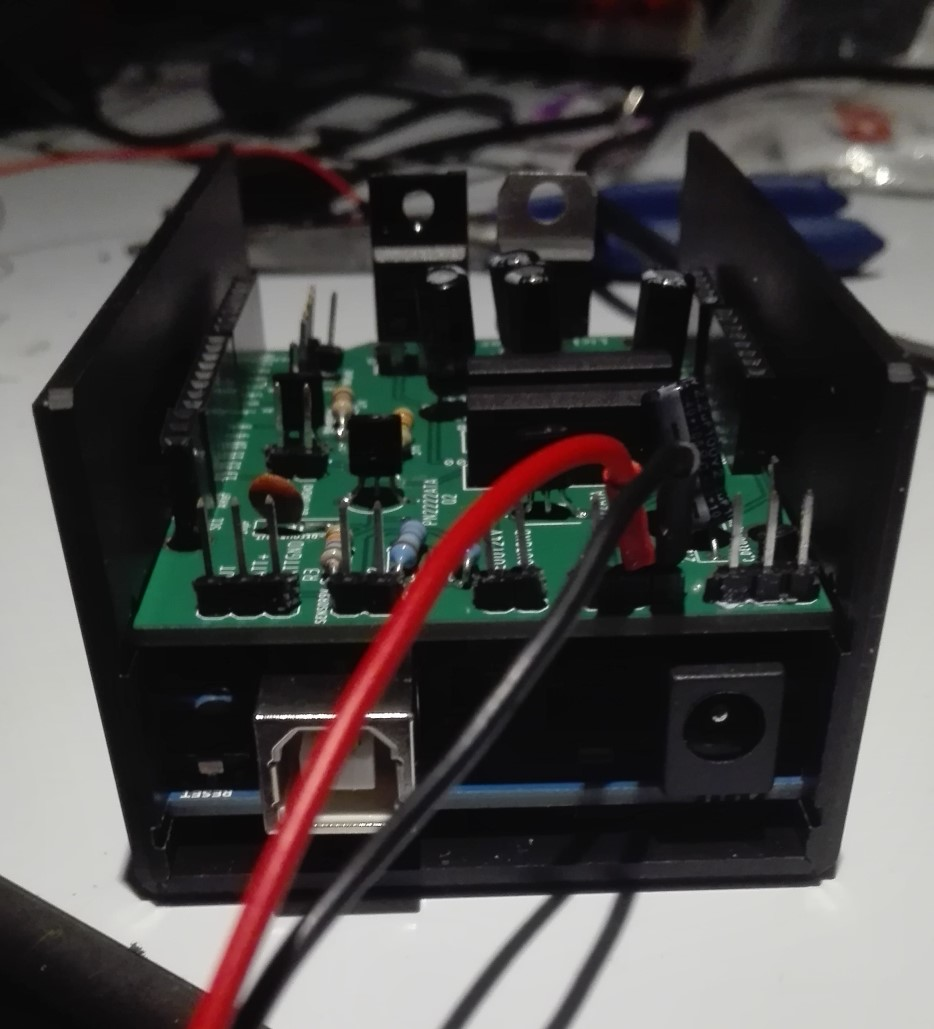
\includegraphics[width=7cm]{images/enclosure.jpg}
    \caption{Design V1: View of the PCB on top of the Arduino}
    \label{fig:my_label}
\end{figure}

This circuit is shown in appendix \ref{fig:schematic}.

\newpage
\subsection{Full design V2}
A second version of the circuit has been designed but not produced. It implemented solutions to some of the problems presented here above.

The 24V relay is replaced by a FET and a flyback diode is added on the load.
The schematic is shown in section \ref{schematicV2}.

\begin{figure}[h!t!b!]
    \centering
    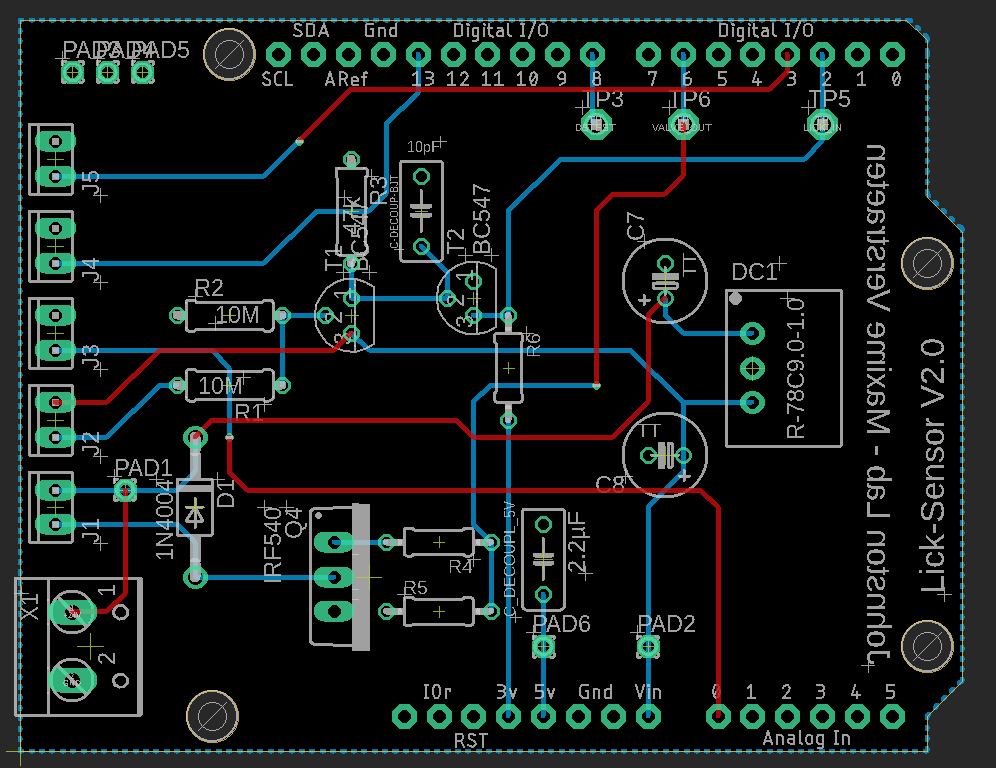
\includegraphics[width = 8cm]{images/schematicV2.PNG}
    \caption{Design V2: PCB view}
    \label{fig:PCBV2}
\end{figure}

\subsection{Full design V3}
\label{designV3}
To add the new valve and bring some of the improvements discussed here-above, a third version of the PCB has been designed and produced.

The new circuit implements, among other things:
\begin{itemize}
    \item An open collector output signal for the motion sensor. This increases the reliability of this part of the circuit as well as its lifetime expectancy and reduce the cost because the Reed relay is replaced by a BJT.
    \item A MOSFET driven actuation of the valve (IRL540) which greatly increases the reliability (the reed relay was especially sensitive at 24V with peak voltage due to the solenoid valve). This does not reduce the cost as logic-level FET is expensive (~£2 for IRL540 on RS and ~1.15 for a relay on Farnell).
    \item Additional fly-back diode instead of RC circuit for the valve recovery. Should be more effective.
    \item Capacitors C7 and C8 are optional. Indeed, the TSR 1-2490 DC/DC converter comes with integrated filtering capacitors. However, if it is replaced by another one that does not comes with capacitors, the pad is present on the PCB. Moreover, they can still be added if additional filtering is required.
\end{itemize}

\begin{figure}[h!t!b!]
    \centering
    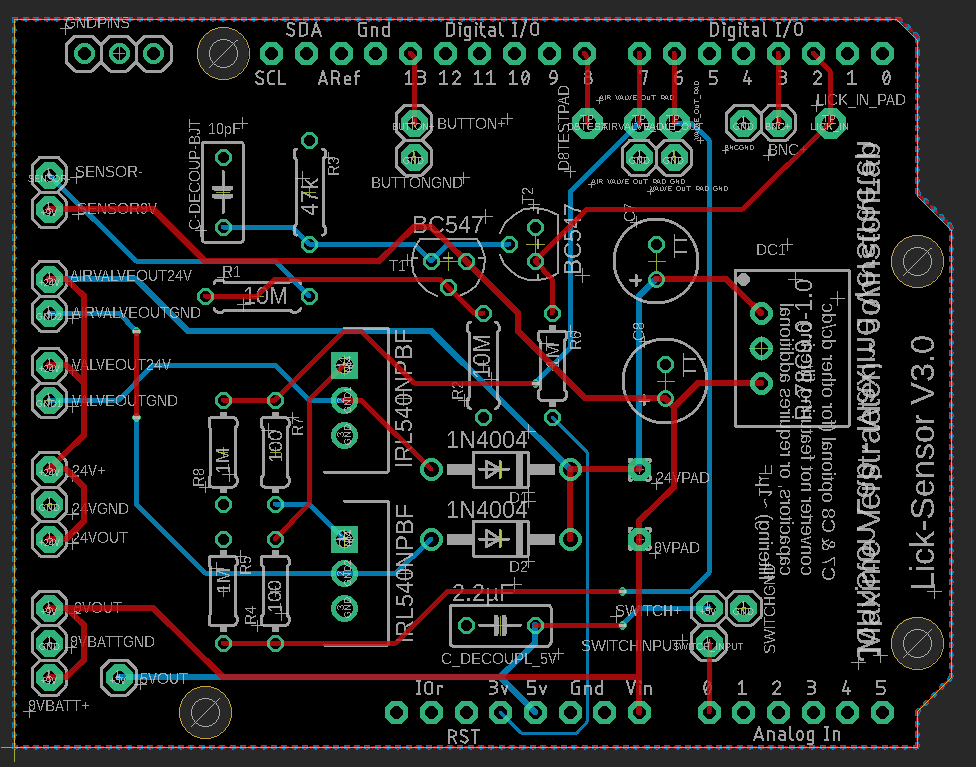
\includegraphics[width = 8cm]{images/BoardViewV3.PNG}
    \caption{PCB V3}
    \label{fig:PCBV3}
\end{figure}

The Eagle files are available on request and the schematic is shown in appendix \ref{schematicV3}.
The PCB is shown on Figure \ref{fig:PCBV3}.

\newpage
\section{Improvements}
\subsection{Zener Diode}
A Zener diode can be used to control the voltage and make sure that no change in sensitivity appears as voltage decreases in case of a battery-powered application. It could also be used as a voltage regulator for the DC Supply.

Another Zener diode coud also be added at the MOSFET gate to protect it from high voltage. In normal operations though, the gate is connected to the Arduino pin which will not output more than 3.3V and 150mA max. Still, ESD could happen so it would be good practice to add it, even though the Arduino also probably features ESD-protection diodes.

\subsection{Reduce the current flowing through the mouse}
R1 and R2 could be increased (20M ohms) to reduce current flowing through the subject but reduces reliability.
TODO MEASURE CURRENT FLOWING

\subsection{FET instead of BJT ?}
Transistors used in the sensor design are BJT wich are okay in a low current application but FET could probably do, even if the voltage-controlled is less convenient than BJT's current-controlled.
The MOSFETs present high input impedance, less fabrication dispersion, very small, easy to scale.
BJTs present input capacitance (bad for HF), higher output resistance (not suited for low-impedance load), lower gain/stage so SNR quickly degrades, current-operated -> higher consumption

In the end, we could use MOSFET to reduce the consumption but this is not necessary.
Additionaly, FETs are harder to use at logic gate signal (need to use FETs like IRL540 which are more expensive).

\subsection{Avoid shorts with stackable design}
One of the issues I ran into, was that my power pins were spatially close (on top) of the Arduino USB Frame (connected to ground). This may have cause a short-circuit between 24V or 9V and Ground. One solution would be to spatially move those pins in another place.
The other solution which I did was to add one more layer of stackable header to further separate the PCB and the µC. This also allows more air to cool both the PCB and the Arduino down.

\subsection{MTA connectors}
Once the design is tested and validated, we can also implement some MTA connectors instead of the pin headers. This will however increase the cost of the design but it might be interesting if the device is shared to other people.

\subsection{Additional valves to control different reward liquids}
Additional valves and tanks could be placed before the main valve so that different liquids can be tested (e.g. sugar and artificial sweetener).
The Uno have some pins available on the shield and they can be used to control another valve actuator circuit (section \ref{actuator}).

\newpage
\section{Troubleshooting}
Note: several ground pins are available on the PCB for easy measurements.
\subsection{The valve doesn't activate}
Make sure that the device is powered by 24V DC.
Check if the valve is opened or closed by putting water in the water tank above.
If it is open check the subsection \ref{staysOpen}.
If it stays closed, check with an oscilloscope (or voltmeter) if 24V is sent to the valve when push-button is pressed. If it is the case and no water is flowing through, the valve might be blocked due to residues (sugars, ions deposit, ... in the valve). Simply try to apply more pressure to the water (blowing hard on the water syringe might do the trick) to try and unclog it.
\subsection{The valve stays open}
\label{staysOpen}
If the valve is always open, check that the switch on the box is on low position. Indeed, if it is up, the valve will stay open.

If the valve still stays open, check with an oscilloscope if a 24V signal is sent to the valve (you can use the BNC output). If the switch is low, and no button is pressed, the signal should be ground. If it stays to 24V no matter what, the valve activation circuit (section \ref{actuator}) might be malfunctioning. Check the voltage on the MOSFET gate to ensure its proper operation.

\subsection{Push-button/switch doesn't work}
Unscrew the box and check that the wires (2 for the push-button (digital signal pulled up and ground); 3 for the switch (5V, ground, signal)) are still in place both on the button itself and on the PCB pins.
If so, plug the USB into the Arduino and open the Serial monitor. When a button is activated, a corresponding message should appear in the Serial monitor (Note: the Serial should be set to 500000 bauds).

\subsection{Is there a polarity for the sensor?}
One of the sensor is connected to 9V and therefore should not be touching any ground. 
The other sensor is connected to ground through a series of resistors.

\subsection{The droplet won't get sucked using the second valve}
Make sure to place the valve below the needle otherwise the capillarity will just stop when air will enter the circuit and the droplet will fall.

\newpage
\appendix

\section{Bill of materials}
The bill of materials is available on the Excel files on my Github: \url{https://github.com/maverstr/Lick-Sensor}

\section{Power dissipation by linear voltage regulators}
The first design used linear voltage regulators to transform the 24V to 9V able to power the Arduino.
They transform excessive voltage in heat.
Therefore the power dissipated = ((24V-15V)+(15V-9V))*Imax
Imax =  1.095V/20ohms (current measurement with voltage meter) = 55mA.

Safety measure : 100mA.

So we get power dissipated = 1.5W
Or 900mW for the first regulator and 600mW for the second one.
The regulators comes within a TO-220 package which is fine for under 1W of dissipation (rule of thumb). However, in a closed box, there will be no airflow.

The datasheet of the regulators specify 60°C/W as thermal resistance for junction/ambient.

\begin{figure}[h!]
    \centering
    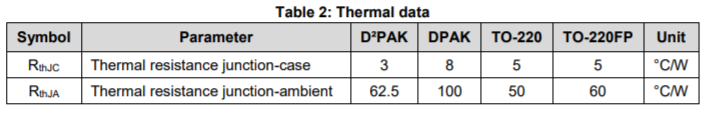
\includegraphics[width = 10cm]{images/thermalData.png}
    \caption{Thermal Data}
    \label{fig:thermalData}
\end{figure}

So at 900mW it's 54°C above ambient. Worst case ambient would be 40°C room temp + enclosed box.. Estimates about 60°C. That makes a total of 104°C.

The datasheet mentions that the maximum operation temperature is 125°C. So we're just under.


\begin{figure}[h!]
    \centering
    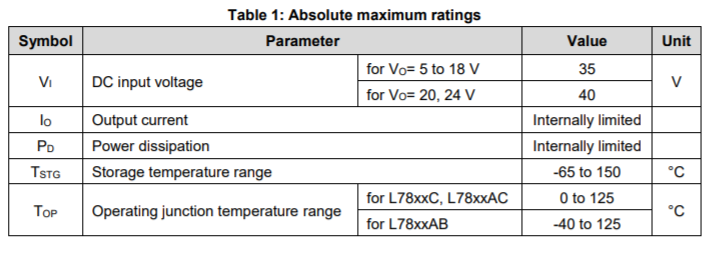
\includegraphics[width = 10cm]{images/thermalData2.png}
    \caption{Maximum operating temperature}
    \label{fig:thermalData2}
\end{figure}

The idea was therefore to drill some holes for the air to flow through the box and monitor the temperature. If it rose too high, a fan was to be added (required 9V and 5V pins were already present on the PCB).

On the PCB: I obtained 1.130V/20ohms = 57mA, as expected.

A simpler and more reliable solution (as the device is used with other devices around, for long term use, by people without skills in electronics) was to replace the linear regulators by DC/DC switching regulators, way more efficient but more expensive.

\newpage

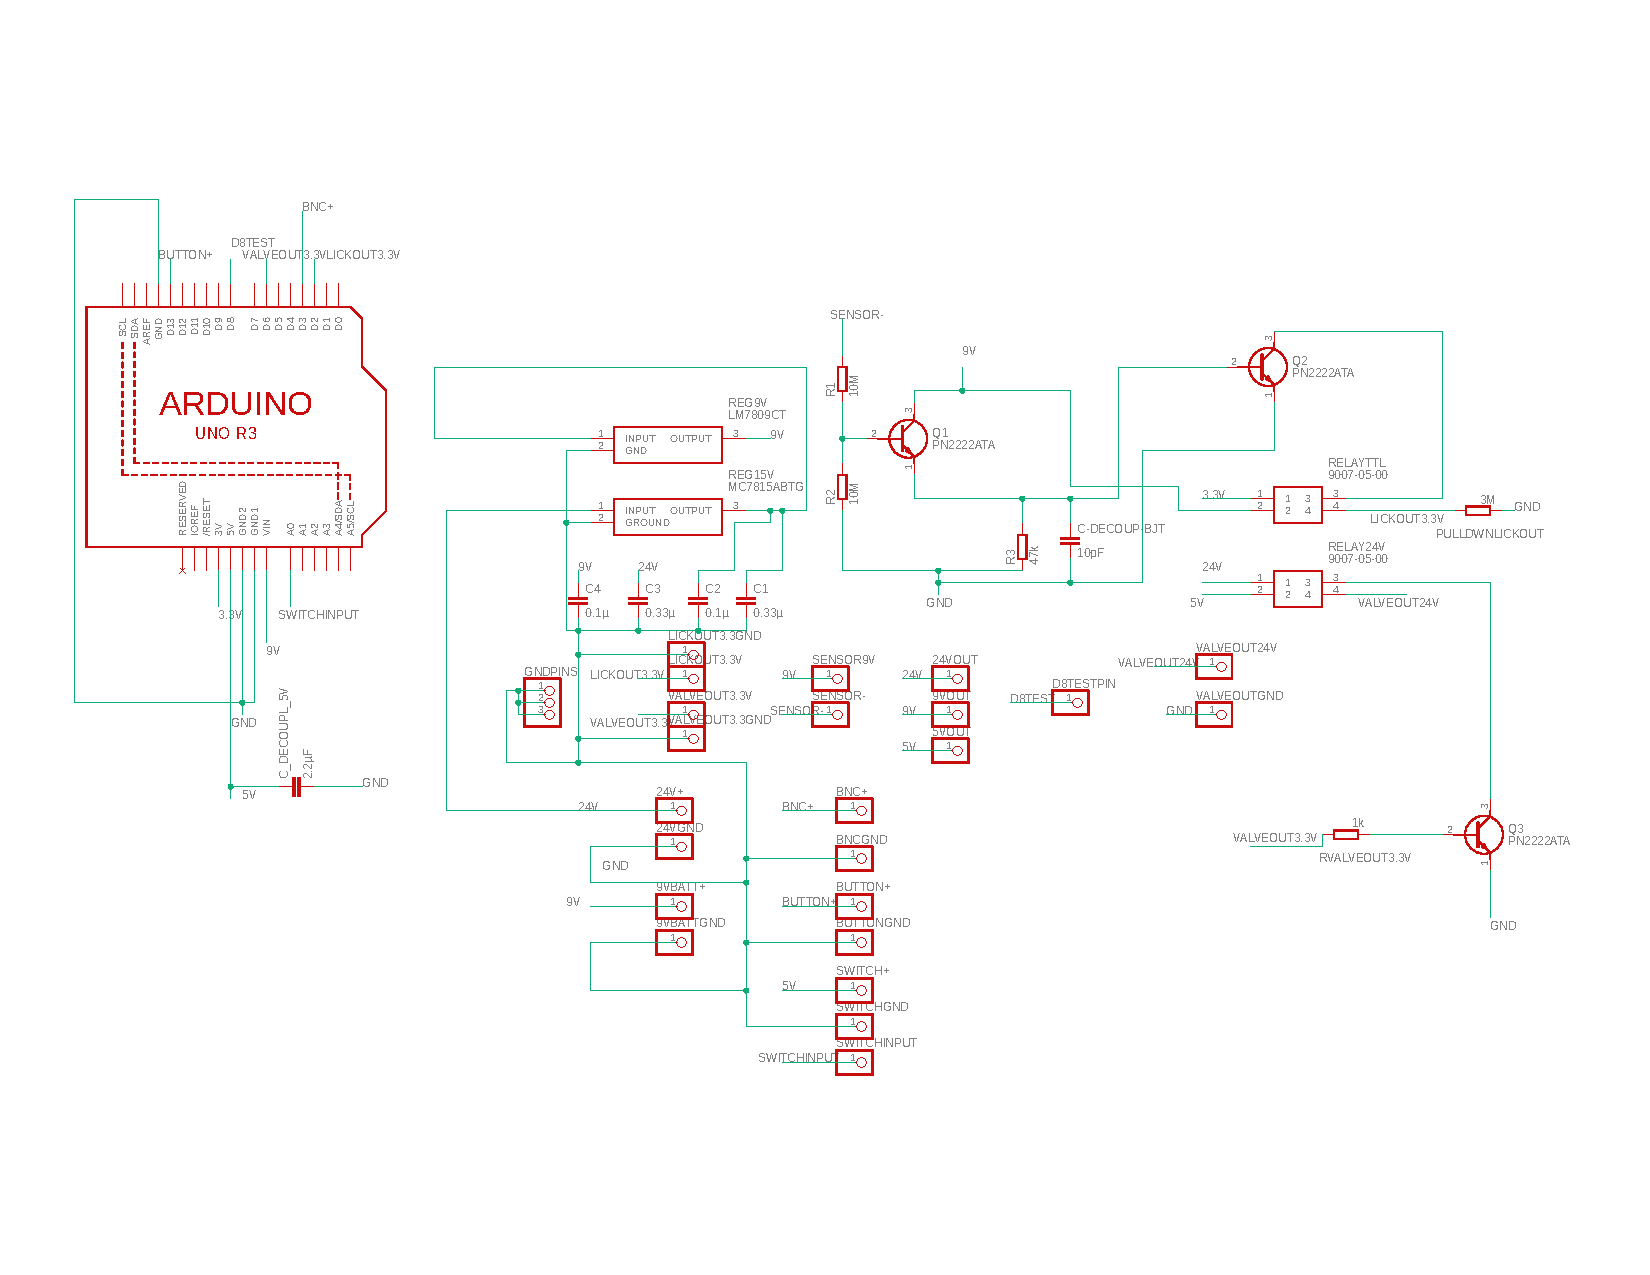
\includepdf[pagecommand= \section{V1: PCB Schematic \label{schematic}}, scale = 1, angle = 270]{images/schematic}


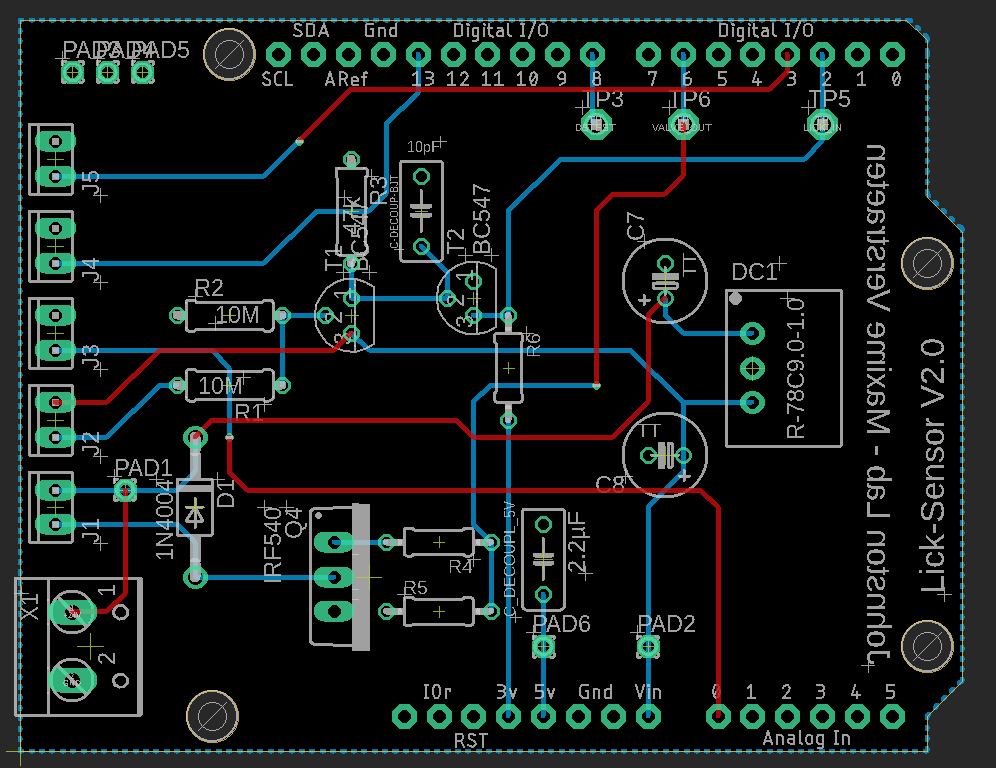
\includepdf[pagecommand= \section{V2: PCB Schematic \label{schematicV2}},scale = 1.2,angle = 270, ]{images/schematicV2}



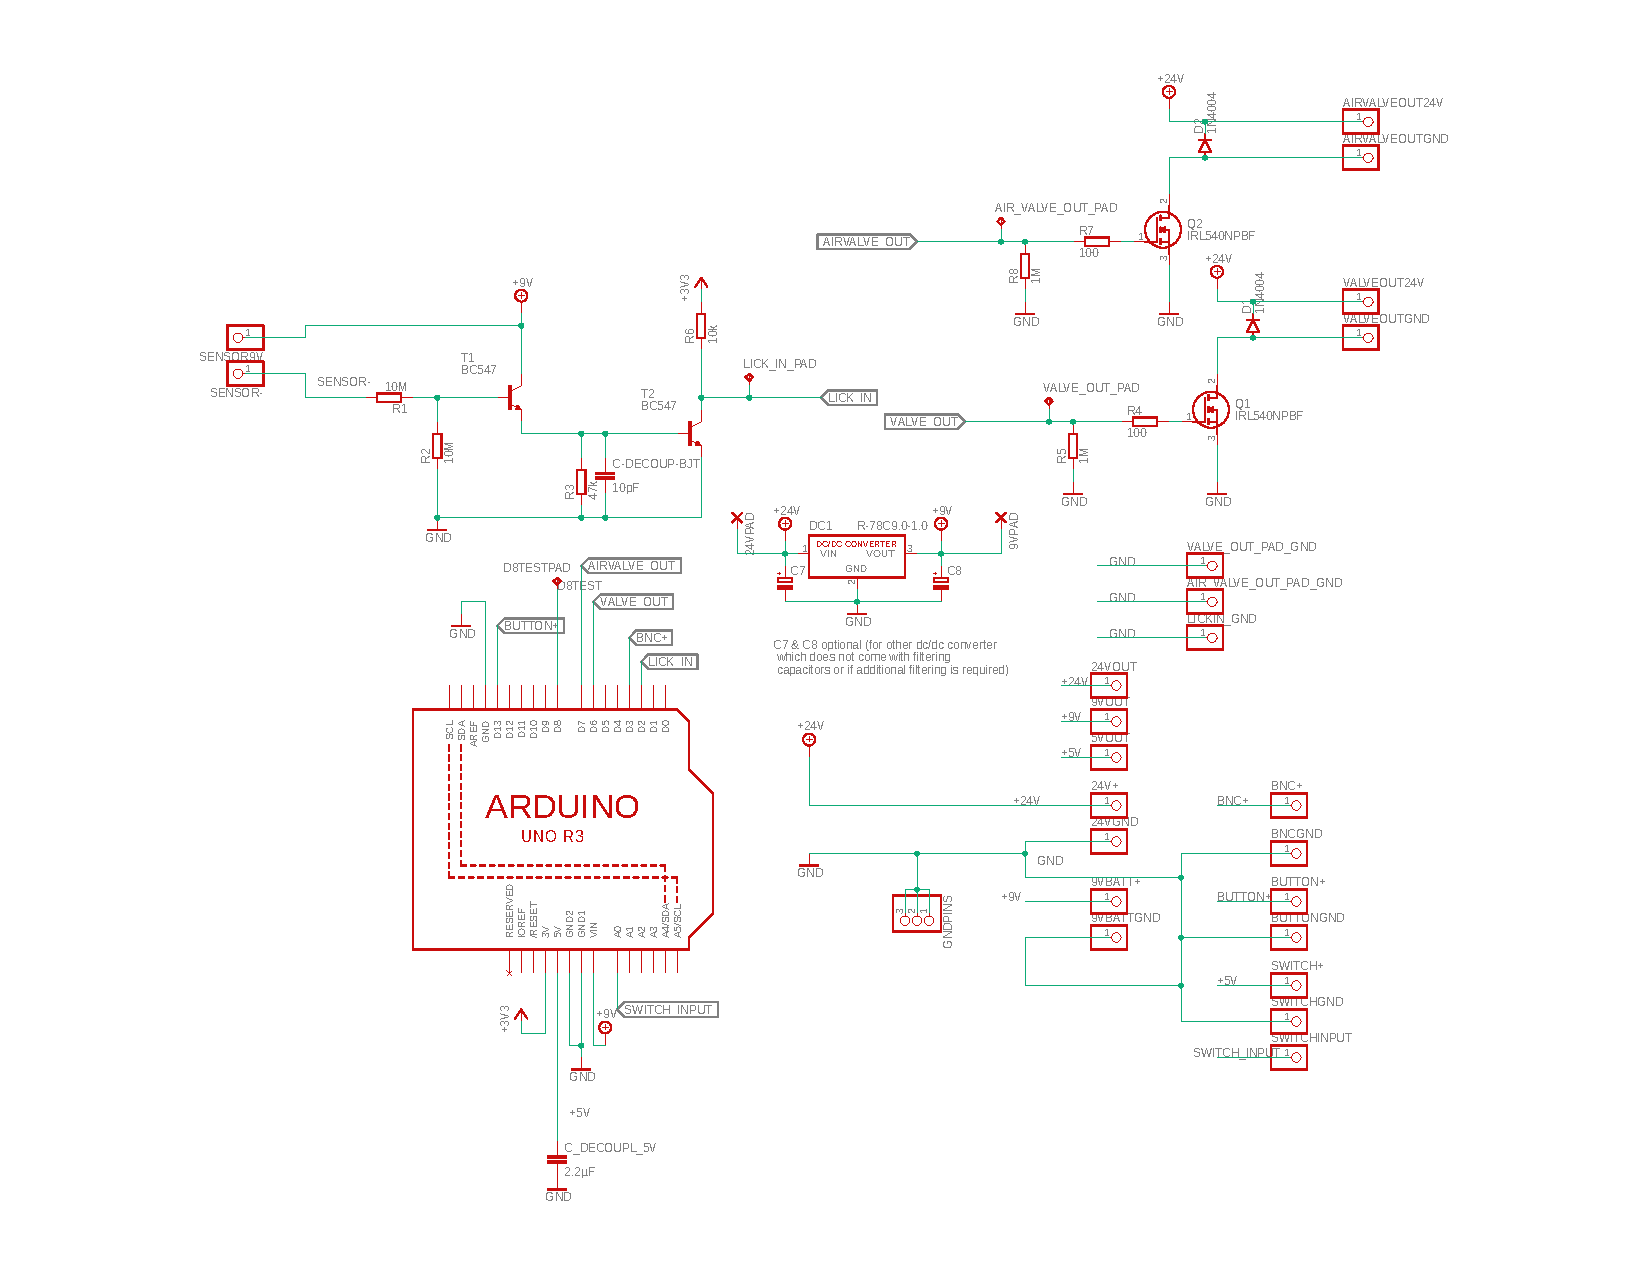
\includepdf[pagecommand= \section{V3: PCB Schematic \label{schematicV3}},scale = 0.85,angle = 270, ]{images/schematicV3}

\bibliographystyle{alpha}
\bibliography{biblio}

\end{document}